%------------------------------------------%
% Cannabis Data Science
% Saturday Morning Statistics
% Date: 3/19/2022
%------------------------------------------%
\documentclass[xcolor={dvipsnames}]{beamer}
\hypersetup{pdfpagemode = FullScreen}
\mode<presentation>{
  \usetheme{Boadilla}
  \usecolortheme{orchid}
  \usefonttheme{default}
  \setbeamertemplate{navigation symbols}{}
  \setbeamertemplate{caption}[numbered]
}
\setbeamersize{
  text margin left = 0.5in,
  text margin right = 0.5in
}

%------------------------------------------%
% Title
%------------------------------------------%
\author{Cannabis Data Science}
\title[\textbf{Saturday Morning Statistics \#16}]{}
\institute[]{\Large Saturday Morning Statistics \#16}
\date{March \nth{19}, 2022}

%------------------------------------------%
% Packages
%------------------------------------------%
\usepackage[english]{babel}
\usepackage[utf8x]{inputenc}
\usepackage{tikz}
\usepackage{xparse}

%------------------------------------------%
% Colors
%------------------------------------------%
\definecolor{Green}{RGB}{34, 153, 84}
\definecolor{LightGreen}{RGB}{218, 247, 166}
\definecolor{DarkGreen}{RGB}{2, 48, 32}
\definecolor{Orange}{RGB}{255, 87, 51}
\definecolor{DarkOrange}{RGB}{199, 0, 57}
\definecolor{Yellow}{RGB}{255, 195, 0}

%------------------------------------------%
% Theme
%------------------------------------------%
\setbeamercolor*{palette primary}{bg=LightGreen, fg=DarkGreen}
\setbeamercolor*{palette secondary}{bg=LightGreen, fg=DarkGreen}
\setbeamercolor*{palette tertiary}{bg=LightGreen, fg=DarkGreen}

%------------------------------------------%
% Packages
%------------------------------------------%
\usepackage{amsmath}
\renewcommand*\footnoterule{} % No separating line on footnote.
\usepackage{mathtools} % For annotating equations.
\usepackage{hhline} % for double bars.
\usepackage[super]{nth} % For formatting 1st, 2nd, 3rd, etc.
\usepackage{graphicx, caption, subcaption}
\usepackage{setspace}

%------------------------------------------%
% Commands
%------------------------------------------%

% Top space.
\newcommand\T{\rule{0pt}{2.5ex}}

% Bottom space.
\newcommand\B{\rule[-1.25ex]{0pt}{0pt}}

% Blocks.
\newenvironment<>{Block}[2][.9\textwidth]
  {\setlength{\textwidth}{#1}
  \begin{actionenv}#3
    \def\insertblocktitle{#2}\par
    \usebeamertemplate{block begin}}
  {\par\usebeamertemplate{block end}
  \end{actionenv}}

% Balls.
\defbeamertemplate{enumerate item}{largeball}
{\begin{pgfpicture}{-1ex}{-0.65ex}{1.5ex}{1.5ex}
\usebeamercolor[fg]{item projected}
{\pgftransformscale{2.5}\pgftext{\Large\pgfuseshading{bigsphere}}}
{\pgftransformshift{\pgfpoint{0pt}{0.5pt}}
\pgftext{\usebeamerfont*{item projected}\small\insertenumlabel}}
\end{pgfpicture}}

% Fancy arrows.
\NewDocumentCommand\UpArrow{O{2.0ex} O{black}}{%
   \mathrel{\tikz[baseline] \draw [->, line width=0.5pt, #2] (0,0) -- ++(0,#1);}} % Fancy up-arrow.
\NewDocumentCommand\DownArrow{O{2.0ex} O{black}}{%
   \mathrel{\tikz[baseline] \draw [<-, line width=0.5pt, #2] (0,0) -- ++(0,#1);}} % Fancy down-arrow.

% Equations with numbers on the left.
\makeatletter
\newcommand{\LeftEqNo}{\let\veqno\@@leqno}
\makeatother

%------------------------------------------%
% Presentation
%------------------------------------------%
\begin{document}

%------------------------------------------%
% Title Page
%------------------------------------------%
\begin{frame}{}
  
\includegraphics[scale=0.33]{images/logo.pdf}
  \vspace*{-2\baselineskip}
  \titlepage
\end{frame}

%------------------------------------------%
% Statistical History
%------------------------------------------%

% Optional: Add a bit of statistical history.


%------------------------------------------%
% Introduction
%------------------------------------------%
\section{Introduction}
\begin{frame}{}

% Question of the day
\begin{center}
\begin{minipage}{.9\linewidth}
\begin{Block}{Question of the day.}

\vspace{.5\baselineskip}
\begin{itemize}

\item Can we apply {\bfseries survival analysis} to study the question: what affects the likelihood of a cultivator, processor, or retailer being successful? Hypothesized effects may include:

\begin{itemize}

\vspace{0.33\baselineskip}

\item Average THC concentration of products;

\vspace{0.33\baselineskip}

\item Rent in the zip code;

\vspace{0.33\baselineskip}

\item Your ideas?

\vspace{0.33\baselineskip}

\end{itemize}

\end{itemize}

\vspace{.5\baselineskip}

\end{Block}
\end{minipage}
\end{center}

\end{frame}


\begin{frame}{Survival Analysis}

\vspace{0.25\baselineskip}

First, define

\vspace{0.5\baselineskip}
\begin{itemize}

\item The \underline{amount of time} individual $i$ has been at risk at time $j$ is $t_{ij}$.

\vspace{0.5\baselineskip}

\item An indicator variable to denote if an individual $i$ has \underline{exited}

$$
d_{ij} = \begin{cases}
&1 \hspace{1ex} \text{\footnotesize if individual} \hspace{1ex} i \hspace{1ex} \text{\footnotesize exited in period} \hspace{1ex} j, \\
&0 \hspace{1ex} \text{\footnotesize otherwise}.
\end{cases}
$$

\end{itemize}

\vspace{0.5\baselineskip}
The chances of individual $i$ surviving period $j$ is given by the {\bfseries survival function}

\vspace{-0.75\baselineskip}
$$
S(t_{ij}) = P(T > t_{ij}).
$$

\vspace{0.5\baselineskip}
The instantaneous risk of failure for individual $i$ in period $j$ is the {\bfseries hazard rate}

\vspace{-0.75\baselineskip}
$$
\lambda(t) = \frac{S^\prime(t)}{S(t)}.
$$

\end{frame}

%------------------------------------------%
% Kaplan–Meier estimator
%------------------------------------------%
\begin{frame}{}

\vspace{1\baselineskip}
{\large \textbf{Kaplan--Meier Estimator}}\vspace{0.75\baselineskip}\\

\begin{minipage}{0.55\textwidth}

\begin{itemize}

\item Used to estimate \underline{survival functions}.

\vspace{0.75\baselineskip}

\item One of the most frequently used methods of survival analysis.

\vspace{0.75\baselineskip}

\end{itemize}

\end{minipage}\hspace{0.05\textwidth}%
\begin{minipage}{0.4\textwidth}

\begin{figure}
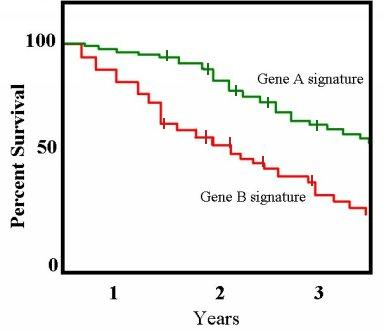
\includegraphics[width=\textwidth]{images/km-plot.jpg}
\end{figure}

\end{minipage}


\begin{itemize}

\item The estimator is given by

$$
\hat{S}(t) = \sum_{t_i=0}^{t_i\leq t}\left(1 - \frac{d_i}{n_i}\right)
$$

where

\vspace{0.25\baselineskip}
\begin{itemize}
\item $t_i$ is exposure time,
\vspace{0.25\baselineskip}
\item $d_i$ is the number of events at time $t_i$,
\vspace{0.25\baselineskip}
\item $n_i$ is the number of individuals surviving through time $t_i$.
\end{itemize}

\end{itemize}

\end{frame}

%------------------------------------------%
% Nelson–Aalen estimator
%------------------------------------------%
\begin{frame}{}

\vspace{1\baselineskip}
{\large \textbf{Nelson--Aalen Estimator}}\vspace{0.75\baselineskip}\\

\begin{minipage}{0.35\textwidth}
An estimator of the \underline{cumulative hazard rate function} given {\itshape censored data} or {\itshape incomplete data}.

\vspace{0.75\baselineskip}

\end{minipage}\hspace{0.2\textwidth}%
\begin{minipage}{0.45\textwidth}

\begin{figure}
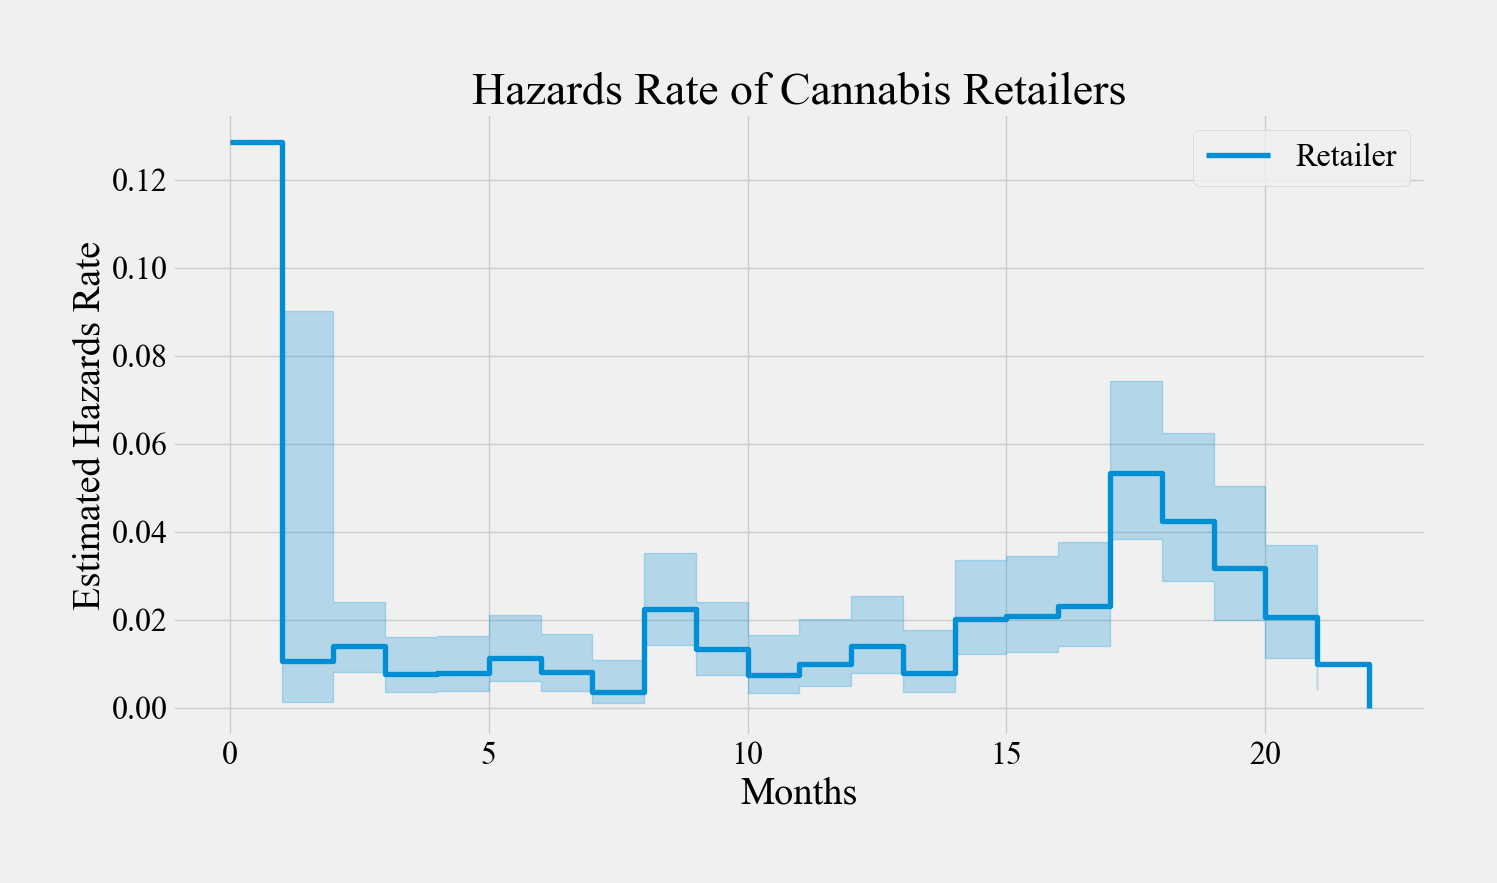
\includegraphics[width=\textwidth]{images/retailer-hazards-rate.png}
\end{figure}

\end{minipage}

\begin{itemize}

\vspace{2\baselineskip}

\item The estimator is given by
$$
\hat{H}(t) = \sum_{t_i=0}^{t_i\leq t} \frac{d_i}{n_i}
$$

\vspace{-0.5\baselineskip}
where

\vspace{0.25\baselineskip}
\begin{itemize}
\item $t_i$ is exposure time,
\vspace{0.25\baselineskip}
\item $d_i$the number of events at time $t_i$,
\vspace{0.25\baselineskip}
\item $n_i$ is the number of individuals surviving through time $t_i$.
\end{itemize}

\end{itemize}

\end{frame}

%------------------------------------------%
% Poisson regressions to estimate hazards models
%------------------------------------------%
\begin{frame}{Poisson regressions to estimate hazards models}

\vspace{0.5\baselineskip}

\begin{minipage}{0.5\textwidth}

You can approximate $d_{ij}$ with a {\bfseries Poisson distribution}

\vspace{-1\baselineskip}
$$
d_{ij} \sim \text{Po}(\mu_{ij}) = \frac{\mu_{ij\exp(-\mu_{ij})}^{d_{ij}}}{d_{ij}!}
$$

with means
$$
\mu_{ij} = t_{ij}\lambda_{ij}.
$$

\end{minipage}\hspace{0.05\textwidth}%
\begin{minipage}{0.45\textwidth}

\begin{figure}
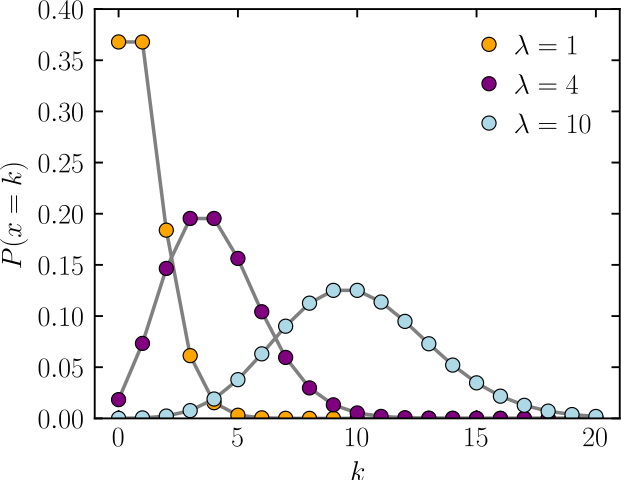
\includegraphics[width=\textwidth]{images/Poisson-distribution.png}
\end{figure}

\end{minipage}

\vspace{2\baselineskip}
The risk incurred by individual $i$ in period $j$ is

$$
\lambda_{ij} = \lambda_j\exp(X_i\beta).
$$

\end{frame}


%------------------------------------------%
% Cox's proportional hazards model
%------------------------------------------%
\begin{frame}{}

\vspace{1\baselineskip}
{\large \textbf{Cox's Proportional Hazards Model}}\vspace{0.75\baselineskip}\\

Given covariates, $X_i$, and parameters, $\beta$, the hazard rate is modeled as

\vspace{-0.5\baselineskip}
$$
\lambda(t) = \lambda_0(t)\text{exp}(X_i\beta),
$$

\vspace{0.5\baselineskip}
where $\lambda_0(t)$ is the baseline hazard. Taking the log yields a \underline{Poisson log-linear model}

$$\text{log}\mu_{ij} = \text{log}t_{ij} + \alpha_j + X_i^\prime \beta.$$

\vspace{0.5\baselineskip}

A 1 unit increase in $X_i$ is interpreted as a change in the average (and median) survival by a factor of $\exp(\beta)$.

\end{frame}


%------------------------------------------%
% Time-dependent Effects
%------------------------------------------%
\begin{frame}{}

\vspace{1\baselineskip}
{\large \textbf{Hazards Model with Time-varying Covariates}}\vspace{0.75\baselineskip}\\

Adding \underline{time-varying covariates} to the hazards model yields

$$\text{log}\lambda_{ij} = \alpha_j + \beta X_{ij},$$

where $X_{ij}$ are the values of the covariates of individual $i$ in interval $j$.

\vspace{1\baselineskip}
{\large \textbf{Hazards Model with Time-dependent Effects}}\vspace{0.75\baselineskip}\\

Adding \underline{time-dependent covariates} to the hazards model yields

$$\text{log}\lambda_{ij} = \alpha_j + \beta_j X_{ij},$$

where $\beta_j$ is the effect of the hazard during interval $j$.


\vspace{1\baselineskip}

{\footnotesize Note: Effects vary only at interval boundaries.}

\end{frame}


%------------------------------------------%
% Cox's proportional hazards model - Bayesian inference
%------------------------------------------%
\begin{frame}{}

\vspace{1\baselineskip}
{\large \textbf{Bayesian Inference of Hazards Model}}\vspace{0.75\baselineskip}\\

\begin{enumerate}

\item First, you specify your priors for the parameters

\vspace*{-1.25\baselineskip}
\begin{align*}
\beta &\sim \mathcal{N}(\mu_\beta, \sigma_\beta^2) \\
\sigma_\beta &\sim \mathcal{U}(a, b) \\
\lambda_j &\sim \Gamma(\alpha, \beta)
\end{align*}

with hyperparameters $\mu_\beta$, $a$, $b$, $\alpha$, and $\beta$.

\vspace{0.75\baselineskip}

\item Second, you simulate draws from the posterior distributions.

\vspace{0.75\baselineskip}

\item Finally, you analyze and interpret your Bayesian estimates.

\end{enumerate}


\end{frame}

% TODO: Further explain Bayesian derivation of posteriors.


%------------------------------------------%
% Takeaway
%------------------------------------------%
\section{Takeaway}
\begin{frame}{}

\begin{center}
\begin{minipage}{3.85in}

% Thank you.
\begin{center}

\includegraphics[width=.25in]{images/prayer.png} {\Large \textbf{Thank you for coming.}}\\
\end{center}
\vspace*{0.5\baselineskip}

% Re-cap the lesson of the week.
\begin{center}
\begin{minipage}{\linewidth}
\begin{Block}{Lessons of the Day}

\vspace{0.5\baselineskip}

\begin{itemize}

\item Survival analysis can help identify factors that \underline{are} and \underline{are not} related to licensees exiting and their chances of surviving.

\vspace{0.5\baselineskip}

\end{itemize}

\end{Block}
\end{minipage}
\end{center}

\vspace*{2\baselineskip}

\end{minipage}
\end{center}

\end{frame}


%------------------------------------------%
% Fin.
%------------------------------------------%
\end{document}
